\documentclass[10pt]{article}
\usepackage[margin=1.0cm]{geometry}
\usepackage[T1]{fontenc}
\usepackage{lmodern}
\usepackage{xcolor}
\usepackage{tikz}
\usepackage{pgfplots}
\usepgfplotslibrary{statistics}
\pgfplotsset{compat=1.18}
\definecolor{srblue}{HTML}{2F6B9A}
\definecolor{opencvorange}{HTML}{D97706}
\definecolor{fps2blue}{HTML}{B9D7EA}
\definecolor{fps5orange}{HTML}{F6C28B}
\definecolor{stslightgreen}{HTML}{A7D8B1}
\definecolor{stsstronggreen}{HTML}{208B3A}
\definecolor{sugarlightpurple}{HTML}{CBB7E8}
\definecolor{sugarstrongpurple}{HTML}{763A9B}
\definecolor{stsedge}{HTML}{1D4E89}
\definecolor{sugaredge}{HTML}{B45309}
\definecolor{incompletegray}{HTML}{9CA3AF}
\definecolor{deltared}{HTML}{B91C1C}
\definecolor{deltagreen}{HTML}{15803D}
\newcommand{\legendcircle}[1]{\tikz[baseline=-0.6ex]\node[draw=black,fill=#1,circle,minimum size=4.5pt,inner sep=0pt] {};}
\newcommand{\legendsquare}[1]{\tikz[baseline=-0.6ex]\node[draw=black,fill=#1,rectangle,minimum size=4.5pt,inner sep=0pt] {};}
\newcommand{\legendtriangle}[1]{\tikz[baseline=-0.6ex]\draw[draw=black,fill=#1,line width=0.4pt] (0,2.3pt)--(-2.3pt,-1.8pt)--(2.3pt,-1.8pt)--cycle;}
\begin{document}
\pagestyle{empty}
\begin{center}
{\Large\bfseries SuGaR-Coarse-9000: Verteilung der Einzelansichten}\\[3pt]
{\small Boxplots und Einzelansichten aus vollständigen Läufen; Farben kodieren das Kameramodell}\\[8pt]
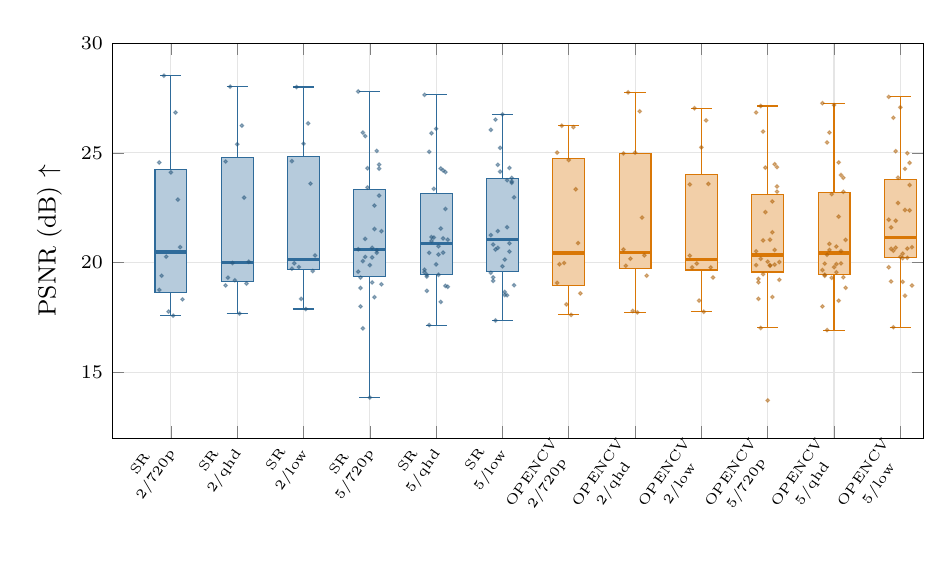
\begin{tikzpicture}
\begin{axis}[height=6.6cm,width=0.98\linewidth,enlarge x limits=0.015,xmin=-0.7,ymin=12,ymax=30,xtick=data,xticklabels={{\shortstack{SR\\2/720p}},{\shortstack{SR\\2/qhd}},{\shortstack{SR\\2/low}},{\shortstack{SR\\5/720p}},{\shortstack{SR\\5/qhd}},{\shortstack{SR\\5/low}},{\shortstack{OPENCV\\2/720p}},{\shortstack{OPENCV\\2/qhd}},{\shortstack{OPENCV\\2/low}},{\shortstack{OPENCV\\5/720p}},{\shortstack{OPENCV\\5/qhd}},{\shortstack{OPENCV\\5/low}}},x tick label style={font=\tiny,rotate=55,anchor=east},ylabel style={font=\small},tick label style={font=\scriptsize},ylabel={PSNR (dB) $\uparrow$},grid=major,grid style={gray!20},xtick={0,1,2,3,4,5,6,7,8,9,10,11},boxplot/draw direction=y]
\draw[fill=srblue!35,draw=srblue] (axis cs:-0.2400,18.65097018) rectangle (axis cs:0.2400,24.22698820);
\draw[draw=srblue,very thick] (axis cs:-0.2400,20.48957667) -- (axis cs:0.2400,20.48957667);
\draw[draw=srblue] (axis cs:0.0000,17.58551062) -- (axis cs:0.0000,18.65097018);
\draw[draw=srblue] (axis cs:0.0000,24.22698820) -- (axis cs:0.0000,28.51558958);
\draw[draw=srblue] (axis cs:-0.1600,17.58551062) -- (axis cs:0.1600,17.58551062);
\draw[draw=srblue] (axis cs:-0.1600,28.51558958) -- (axis cs:0.1600,28.51558958);
\addplot[only marks,mark=*,mark size=0.65pt,color=srblue!80!black,opacity=0.45] coordinates {(-0.17500,18.75836066) (0.03500,17.58551062) (-0.14000,19.40410831) (0.07000,26.83805218) (-0.10500,28.51558958) (0.10500,22.87026125) (-0.07000,20.27302781) (0.14000,20.70612553) (-0.03500,17.77331062) (0.17500,18.32879876) (0.00000,24.11488165) (-0.17500,24.56330787)};
\draw[fill=srblue!35,draw=srblue] (axis cs:0.7600,19.16188258) rectangle (axis cs:1.2400,24.80475288);
\draw[draw=srblue,very thick] (axis cs:0.7600,20.01391262) -- (axis cs:1.2400,20.01391262);
\draw[draw=srblue] (axis cs:1.0000,17.68089817) -- (axis cs:1.0000,19.16188258);
\draw[draw=srblue] (axis cs:1.0000,24.80475288) -- (axis cs:1.0000,28.01625065);
\draw[draw=srblue] (axis cs:0.8400,17.68089817) -- (axis cs:1.1600,17.68089817);
\draw[draw=srblue] (axis cs:0.8400,28.01625065) -- (axis cs:1.1600,28.01625065);
\addplot[only marks,mark=*,mark size=0.65pt,color=srblue!80!black,opacity=0.45] coordinates {(0.82500,18.96176507) (1.03500,17.68089817) (0.86000,19.31546696) (1.07000,26.24267944) (0.89500,28.01625065) (1.10500,22.96280674) (0.93000,19.98525398) (1.14000,19.05152026) (0.96500,19.19867001) (1.17500,20.04257126) (1.00000,25.39495975) (0.82500,24.60801726)};
\draw[fill=srblue!35,draw=srblue] (axis cs:1.7600,19.69761237) rectangle (axis cs:2.2400,24.82529372);
\draw[draw=srblue,very thick] (axis cs:1.7600,20.15068489) -- (axis cs:2.2400,20.15068489);
\draw[draw=srblue] (axis cs:2.0000,17.88810860) -- (axis cs:2.0000,19.69761237);
\draw[draw=srblue] (axis cs:2.0000,24.82529372) -- (axis cs:2.0000,27.99943344);
\draw[draw=srblue] (axis cs:1.8400,17.88810860) -- (axis cs:2.1600,17.88810860);
\draw[draw=srblue] (axis cs:1.8400,27.99943344) -- (axis cs:2.1600,27.99943344);
\addplot[only marks,mark=*,mark size=0.65pt,color=srblue!80!black,opacity=0.45] coordinates {(1.82500,19.72376634) (2.03500,17.88810860) (1.86000,19.97351353) (2.07000,26.34683518) (1.89500,27.99943344) (2.10500,23.60026136) (1.93000,19.80309012) (2.14000,19.61915048) (1.96500,18.35063430) (2.17500,20.32785626) (2.00000,25.42078156) (1.82500,24.62679777)};
\draw[fill=srblue!35,draw=srblue] (axis cs:2.7600,19.38671531) rectangle (axis cs:3.2400,23.33352970);
\draw[draw=srblue,very thick] (axis cs:2.7600,20.58605641) -- (axis cs:3.2400,20.58605641);
\draw[draw=srblue] (axis cs:3.0000,13.85543477) -- (axis cs:3.0000,19.38671531);
\draw[draw=srblue] (axis cs:3.0000,23.33352970) -- (axis cs:3.0000,27.79819017);
\draw[draw=srblue] (axis cs:2.8400,13.85543477) -- (axis cs:3.1600,13.85543477);
\draw[draw=srblue] (axis cs:2.8400,27.79819017) -- (axis cs:3.1600,27.79819017);
\addplot[only marks,mark=*,mark size=0.65pt,color=srblue!80!black,opacity=0.45] coordinates {(2.82500,20.61180710) (3.03500,20.23942775) (2.86000,19.31911821) (3.07000,18.42731743) (2.89500,17.00919308) (3.10500,20.44864329) (2.93000,20.26228063) (3.14000,24.28108654) (2.96500,23.42713277) (3.17500,21.43280179) (3.00000,13.85543477) (2.82500,27.79819017) (3.03500,20.68027149) (2.86000,18.84686504) (3.07000,21.53168969) (2.89500,20.07205231) (3.10500,20.56030573) (2.93000,21.08299037) (3.14000,23.05272050) (2.96500,24.30086054) (3.17500,19.01600858) (3.00000,19.88847243) (2.82500,19.58950663) (3.03500,19.09851830) (2.86000,18.00666821) (3.07000,22.60053600) (2.89500,25.92130505) (3.10500,25.09113967) (2.93000,25.76540129) (3.14000,24.46840447)};
\draw[fill=srblue!35,draw=srblue] (axis cs:3.7600,19.47823901) rectangle (axis cs:4.2400,23.13400984);
\draw[draw=srblue,very thick] (axis cs:3.7600,20.86722540) -- (axis cs:4.2400,20.86722540);
\draw[draw=srblue] (axis cs:4.0000,17.15691446) -- (axis cs:4.0000,19.47823901);
\draw[draw=srblue] (axis cs:4.0000,23.13400984) -- (axis cs:4.0000,27.64434209);
\draw[draw=srblue] (axis cs:3.8400,17.15691446) -- (axis cs:4.1600,17.15691446);
\draw[draw=srblue] (axis cs:3.8400,27.64434209) -- (axis cs:4.1600,27.64434209);
\addplot[only marks,mark=*,mark size=0.65pt,color=srblue!80!black,opacity=0.45] coordinates {(3.82500,19.56505463) (4.03500,20.37056431) (3.86000,19.36702471) (4.07000,18.21038523) (3.89500,17.15691446) (4.10500,20.45643284) (3.93000,21.16525768) (4.14000,24.12778289) (3.96500,23.36375045) (4.17500,21.04647945) (4.00000,26.09927733) (3.82500,27.64434209) (4.03500,19.44930047) (3.86000,18.71570732) (4.07000,21.55409996) (3.89500,20.44736664) (4.10500,21.10796536) (3.93000,20.98775609) (4.14000,18.94365265) (3.96500,21.14183213) (4.17500,18.90380451) (4.00000,19.92413911) (3.82500,19.68190248) (4.03500,20.74669470) (3.86000,19.44650300) (4.07000,24.28864526) (3.89500,25.05019041) (4.10500,24.20371426) (3.93000,25.89676038) (4.14000,22.44478800)};
\draw[fill=srblue!35,draw=srblue] (axis cs:4.7600,19.61217934) rectangle (axis cs:5.2400,23.83486454);
\draw[draw=srblue,very thick] (axis cs:4.7600,21.06851999) -- (axis cs:5.2400,21.06851999);
\draw[draw=srblue] (axis cs:5.0000,17.36796398) -- (axis cs:5.0000,19.61217934);
\draw[draw=srblue] (axis cs:5.0000,23.83486454) -- (axis cs:5.0000,26.75349605);
\draw[draw=srblue] (axis cs:4.8400,17.36796398) -- (axis cs:5.1600,17.36796398);
\draw[draw=srblue] (axis cs:4.8400,26.75349605) -- (axis cs:5.1600,26.75349605);
\addplot[only marks,mark=*,mark size=0.65pt,color=srblue!80!black,opacity=0.45] coordinates {(4.82500,21.25588701) (5.03500,20.14113146) (4.86000,19.33107850) (5.07000,18.51766058) (4.89500,17.36796398) (5.10500,20.50488226) (4.93000,21.43846675) (5.14000,23.63359647) (4.96500,25.22818682) (5.17500,22.97797983) (5.00000,26.75349605) (4.82500,26.04957305) (5.03500,18.66403215) (4.86000,20.82630764) (5.07000,21.61541783) (4.89500,20.60146184) (5.10500,20.88115298) (4.93000,20.67334487) (5.14000,23.86142324) (4.96500,24.14494390) (5.17500,18.97272515) (5.00000,19.83350958) (4.82500,19.53840260) (5.03500,18.52858900) (4.86000,19.17036502) (5.07000,23.75518846) (4.89500,26.51442104) (5.10500,24.31485663) (4.93000,24.45756912) (5.14000,23.69692354)};
\draw[fill=opencvorange!35,draw=opencvorange] (axis cs:5.7600,18.95972695) rectangle (axis cs:6.2400,24.76002508);
\draw[draw=opencvorange,very thick] (axis cs:5.7600,20.43794448) -- (axis cs:6.2400,20.43794448);
\draw[draw=opencvorange] (axis cs:6.0000,17.62030859) -- (axis cs:6.0000,18.95972695);
\draw[draw=opencvorange] (axis cs:6.0000,24.76002508) -- (axis cs:6.0000,26.23653556);
\draw[draw=opencvorange] (axis cs:5.8400,17.62030859) -- (axis cs:6.1600,17.62030859);
\draw[draw=opencvorange] (axis cs:5.8400,26.23653556) -- (axis cs:6.1600,26.23653556);
\addplot[only marks,mark=*,mark size=0.65pt,color=opencvorange!80!black,opacity=0.45] coordinates {(5.82500,19.07871752) (6.03500,17.62030859) (5.86000,19.93031652) (6.07000,26.17326494) (5.89500,26.23653556) (6.10500,23.34320143) (5.93000,19.98460262) (6.14000,20.89128634) (5.96500,18.09988009) (6.17500,18.60275523) (6.00000,24.67576334) (5.82500,25.01281029)};
\draw[fill=opencvorange!35,draw=opencvorange] (axis cs:6.7600,19.74453452) rectangle (axis cs:7.2400,24.98497257);
\draw[draw=opencvorange,very thick] (axis cs:6.7600,20.46358489) -- (axis cs:7.2400,20.46358489);
\draw[draw=opencvorange] (axis cs:7.0000,17.73440225) -- (axis cs:7.0000,19.74453452);
\draw[draw=opencvorange] (axis cs:7.0000,24.98497257) -- (axis cs:7.0000,27.75987647);
\draw[draw=opencvorange] (axis cs:6.8400,17.73440225) -- (axis cs:7.1600,17.73440225);
\draw[draw=opencvorange] (axis cs:6.8400,27.75987647) -- (axis cs:7.1600,27.75987647);
\addplot[only marks,mark=*,mark size=0.65pt,color=opencvorange!80!black,opacity=0.45] coordinates {(6.82500,20.59702164) (7.03500,17.73440225) (6.86000,19.85726572) (7.07000,26.89407130) (6.89500,27.75987647) (7.10500,22.05263148) (6.93000,20.18129312) (7.14000,20.33014814) (6.96500,17.80097028) (7.17500,19.40634091) (7.00000,25.01104869) (6.82500,24.97628053)};
\draw[fill=opencvorange!35,draw=opencvorange] (axis cs:7.7600,19.66711705) rectangle (axis cs:8.2400,24.00332648);
\draw[draw=opencvorange,very thick] (axis cs:7.7600,20.13806733) -- (axis cs:8.2400,20.13806733);
\draw[draw=opencvorange] (axis cs:8.0000,17.76276638) -- (axis cs:8.0000,19.66711705);
\draw[draw=opencvorange] (axis cs:8.0000,24.00332648) -- (axis cs:8.0000,27.03476767);
\draw[draw=opencvorange] (axis cs:7.8400,17.76276638) -- (axis cs:8.1600,17.76276638);
\draw[draw=opencvorange] (axis cs:7.8400,27.03476767) -- (axis cs:8.1600,27.03476767);
\addplot[only marks,mark=*,mark size=0.65pt,color=opencvorange!80!black,opacity=0.45] coordinates {(7.82500,20.31667512) (8.03500,17.76276638) (7.86000,19.78864986) (8.07000,26.48138677) (7.89500,27.03476767) (8.10500,23.58713222) (7.93000,19.95945955) (8.14000,19.78071429) (7.96500,18.27249559) (8.17500,19.32632534) (8.00000,25.25190928) (7.82500,23.56329381)};
\draw[fill=opencvorange!35,draw=opencvorange] (axis cs:8.7600,19.57283861) rectangle (axis cs:9.2400,23.12276198);
\draw[draw=opencvorange,very thick] (axis cs:8.7600,20.34753344) -- (axis cs:9.2400,20.34753344);
\draw[draw=opencvorange] (axis cs:9.0000,17.02689572) -- (axis cs:9.0000,19.57283861);
\draw[draw=opencvorange] (axis cs:9.0000,23.12276198) -- (axis cs:9.0000,27.13444111);
\draw[draw=opencvorange] (axis cs:8.8400,17.02689572) -- (axis cs:9.1600,17.02689572);
\draw[draw=opencvorange] (axis cs:8.8400,27.13444111) -- (axis cs:9.1600,27.13444111);
\addplot[only marks,mark=*,mark size=0.65pt,color=opencvorange!80!black,opacity=0.45] coordinates {(8.82500,20.51976254) (9.03500,19.88454075) (8.86000,19.26138577) (9.07000,18.43643783) (8.89500,17.02689572) (9.10500,19.91012449) (8.93000,19.47697060) (9.14000,23.23416817) (8.96500,22.30398481) (9.17500,20.02691983) (9.00000,13.72496354) (8.82500,26.83989713) (9.03500,21.04292296) (8.86000,18.35416787) (9.07000,21.38370161) (8.89500,20.17530434) (9.10500,20.57971699) (8.93000,21.01371260) (9.14000,23.47263150) (8.96500,24.32951830) (9.17500,19.22099329) (9.00000,20.04457069) (8.82500,19.89085887) (9.03500,19.86044263) (8.86000,19.10671505) (9.07000,22.78854343) (8.89500,27.13444111) (9.10500,24.48468252) (8.93000,25.97337995) (9.14000,24.35128911)};
\draw[fill=opencvorange!35,draw=opencvorange] (axis cs:9.7600,19.47859287) rectangle (axis cs:10.2400,23.20275981);
\draw[draw=opencvorange,very thick] (axis cs:9.7600,20.44334815) -- (axis cs:10.2400,20.44334815);
\draw[draw=opencvorange] (axis cs:10.0000,16.92973659) -- (axis cs:10.0000,19.47859287);
\draw[draw=opencvorange] (axis cs:10.0000,23.20275981) -- (axis cs:10.0000,27.26332470);
\draw[draw=opencvorange] (axis cs:9.8400,16.92973659) -- (axis cs:10.1600,16.92973659);
\draw[draw=opencvorange] (axis cs:9.8400,27.26332470) -- (axis cs:10.1600,27.26332470);
\addplot[only marks,mark=*,mark size=0.65pt,color=opencvorange!80!black,opacity=0.45] coordinates {(9.82500,18.00699692) (10.03500,19.93533540) (9.86000,19.40153819) (10.07000,18.26736053) (9.89500,16.92973659) (10.10500,19.96699864) (9.93000,20.85623067) (10.14000,23.86488166) (9.96500,23.12219144) (10.17500,21.03831821) (10.00000,27.17957062) (9.82500,27.26332470) (10.03500,19.56425406) (9.86000,19.45003914) (10.07000,22.09804953) (9.89500,20.35882822) (10.10500,20.52786809) (9.93000,20.57791237) (10.14000,19.33505663) (9.96500,19.30764459) (10.17500,18.85492585) (10.00000,19.79396001) (9.82500,19.66427055) (10.03500,20.73457426) (9.86000,19.95720494) (10.07000,24.56463855) (9.89500,25.47432466) (10.10500,23.98963639) (9.93000,25.92771287) (10.14000,23.22961594)};
\draw[fill=opencvorange!35,draw=opencvorange] (axis cs:10.7600,20.23344276) rectangle (axis cs:11.2400,23.78707144);
\draw[draw=opencvorange,very thick] (axis cs:10.7600,21.15687647) -- (axis cs:11.2400,21.15687647);
\draw[draw=opencvorange] (axis cs:11.0000,17.05902714) -- (axis cs:11.0000,20.23344276);
\draw[draw=opencvorange] (axis cs:11.0000,23.78707144) -- (axis cs:11.0000,27.55197797);
\draw[draw=opencvorange] (axis cs:10.8400,17.05902714) -- (axis cs:11.1600,17.05902714);
\draw[draw=opencvorange] (axis cs:10.8400,27.55197797) -- (axis cs:11.1600,27.55197797);
\addplot[only marks,mark=*,mark size=0.65pt,color=opencvorange!80!black,opacity=0.45] coordinates {(10.82500,21.95606431) (11.03500,20.20769762) (10.86000,19.14501488) (11.07000,18.48929098) (10.89500,17.05902714) (11.10500,20.22199567) (10.93000,21.90876720) (11.14000,22.38245232) (10.96500,22.71888268) (11.17500,20.70682037) (11.00000,27.07367271) (10.82500,27.55197797) (11.03500,19.12719067) (10.86000,21.60693256) (11.07000,22.39890700) (10.89500,20.54250024) (11.10500,20.64286585) (10.93000,20.68142542) (11.14000,23.53548414) (10.96500,23.87093388) (11.17500,18.96119633) (11.00000,20.26778404) (10.82500,19.79059815) (11.03500,20.40917789) (10.86000,20.63074605) (11.07000,24.27169487) (10.89500,26.60144304) (11.10500,24.98722460) (10.93000,25.07823826) (11.14000,24.54841595)};
\end{axis}
\end{tikzpicture}
\par\vspace{3pt}
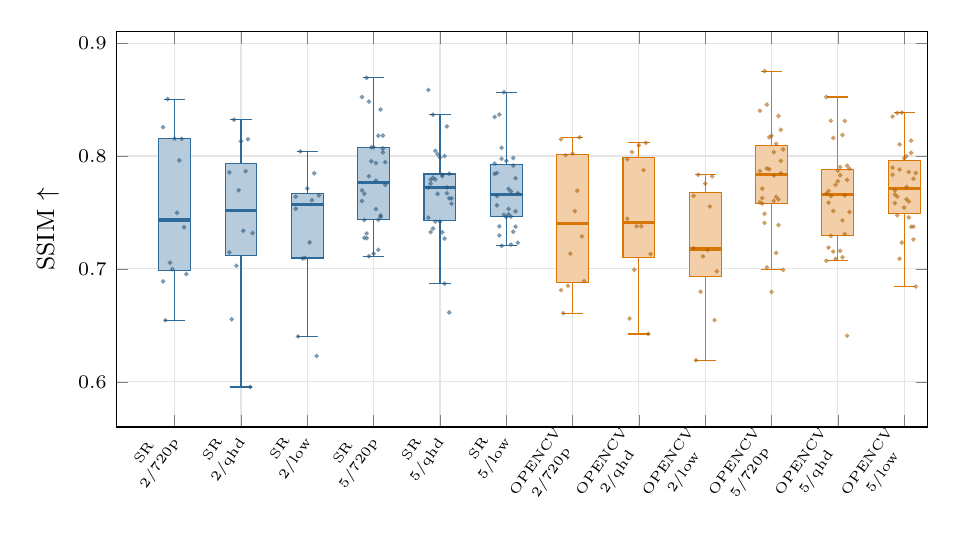
\begin{tikzpicture}
\begin{axis}[height=6.6cm,width=0.98\linewidth,enlarge x limits=0.015,xmin=-0.7,ymin=0.56,ymax=0.91,xtick=data,xticklabels={{\shortstack{SR\\2/720p}},{\shortstack{SR\\2/qhd}},{\shortstack{SR\\2/low}},{\shortstack{SR\\5/720p}},{\shortstack{SR\\5/qhd}},{\shortstack{SR\\5/low}},{\shortstack{OPENCV\\2/720p}},{\shortstack{OPENCV\\2/qhd}},{\shortstack{OPENCV\\2/low}},{\shortstack{OPENCV\\5/720p}},{\shortstack{OPENCV\\5/qhd}},{\shortstack{OPENCV\\5/low}}},x tick label style={font=\tiny,rotate=55,anchor=east},ylabel style={font=\small},tick label style={font=\scriptsize},ylabel={SSIM $\uparrow$},grid=major,grid style={gray!20},xtick={0,1,2,3,4,5,6,7,8,9,10,11},boxplot/draw direction=y]
\draw[fill=srblue!35,draw=srblue] (axis cs:-0.2400,0.69877443) rectangle (axis cs:0.2400,0.81531495);
\draw[draw=srblue,very thick] (axis cs:-0.2400,0.74332234) -- (axis cs:0.2400,0.74332234);
\draw[draw=srblue] (axis cs:0.0000,0.65456408) -- (axis cs:0.0000,0.69877443);
\draw[draw=srblue] (axis cs:0.0000,0.81531495) -- (axis cs:0.0000,0.85046405);
\draw[draw=srblue] (axis cs:-0.1600,0.65456408) -- (axis cs:0.1600,0.65456408);
\draw[draw=srblue] (axis cs:-0.1600,0.85046405) -- (axis cs:0.1600,0.85046405);
\addplot[only marks,mark=*,mark size=0.65pt,color=srblue!80!black,opacity=0.45] coordinates {(-0.17500,0.68898124) (0.03500,0.74971533) (-0.14000,0.65456408) (0.07000,0.79613930) (-0.10500,0.85046405) (0.10500,0.81527662) (-0.07000,0.70549148) (0.14000,0.73692936) (-0.03500,0.69988382) (0.17500,0.69544625) (0.00000,0.81542993) (-0.17500,0.82553470)};
\draw[fill=srblue!35,draw=srblue] (axis cs:0.7600,0.71173091) rectangle (axis cs:1.2400,0.79321270);
\draw[draw=srblue,very thick] (axis cs:0.7600,0.75176784) -- (axis cs:1.2400,0.75176784);
\draw[draw=srblue] (axis cs:1.0000,0.59543335) -- (axis cs:1.0000,0.71173091);
\draw[draw=srblue] (axis cs:1.0000,0.79321270) -- (axis cs:1.0000,0.83216286);
\draw[draw=srblue] (axis cs:0.8400,0.59543335) -- (axis cs:1.1600,0.59543335);
\draw[draw=srblue] (axis cs:0.8400,0.83216286) -- (axis cs:1.1600,0.83216286);
\addplot[only marks,mark=*,mark size=0.65pt,color=srblue!80!black,opacity=0.45] coordinates {(0.82500,0.71469671) (1.03500,0.73380184) (0.86000,0.65536737) (1.07000,0.78657275) (0.89500,0.83216286) (1.10500,0.81493783) (0.93000,0.70283353) (1.14000,0.59543335) (0.96500,0.76973385) (1.17500,0.73177671) (1.00000,0.81313252) (0.82500,0.78556973)};
\draw[fill=srblue!35,draw=srblue] (axis cs:1.7600,0.70965467) rectangle (axis cs:2.2400,0.76665512);
\draw[draw=srblue,very thick] (axis cs:1.7600,0.75709954) -- (axis cs:2.2400,0.75709954);
\draw[draw=srblue] (axis cs:2.0000,0.64024866) -- (axis cs:2.0000,0.70965467);
\draw[draw=srblue] (axis cs:2.0000,0.76665512) -- (axis cs:2.0000,0.80405152);
\draw[draw=srblue] (axis cs:1.8400,0.64024866) -- (axis cs:2.1600,0.64024866);
\draw[draw=srblue] (axis cs:1.8400,0.80405152) -- (axis cs:2.1600,0.80405152);
\addplot[only marks,mark=*,mark size=0.65pt,color=srblue!80!black,opacity=0.45] coordinates {(1.82500,0.76403105) (2.03500,0.72346789) (1.86000,0.64024866) (2.07000,0.76092011) (1.89500,0.80405152) (2.10500,0.78476626) (1.93000,0.70930755) (2.14000,0.62289619) (1.96500,0.70977038) (2.17500,0.76512879) (2.00000,0.77123410) (1.82500,0.75327897)};
\draw[fill=srblue!35,draw=srblue] (axis cs:2.7600,0.74414776) rectangle (axis cs:3.2400,0.80750903);
\draw[draw=srblue,very thick] (axis cs:2.7600,0.77640900) -- (axis cs:3.2400,0.77640900);
\draw[draw=srblue] (axis cs:3.0000,0.71122342) -- (axis cs:3.0000,0.74414776);
\draw[draw=srblue] (axis cs:3.0000,0.80750903) -- (axis cs:3.0000,0.86922091);
\draw[draw=srblue] (axis cs:2.8400,0.71122342) -- (axis cs:3.1600,0.71122342);
\draw[draw=srblue] (axis cs:2.8400,0.86922091) -- (axis cs:3.1600,0.86922091);
\addplot[only marks,mark=*,mark size=0.65pt,color=srblue!80!black,opacity=0.45] coordinates {(2.82500,0.76015162) (3.03500,0.77823234) (2.86000,0.74328625) (3.07000,0.74349475) (2.89500,0.73141307) (3.10500,0.74610680) (2.93000,0.71122342) (3.14000,0.80679101) (2.96500,0.79539245) (3.17500,0.77458566) (3.00000,0.71359998) (2.82500,0.85232824) (3.03500,0.79375505) (2.86000,0.76656610) (3.07000,0.71692008) (2.89500,0.72721833) (3.10500,0.74745774) (2.93000,0.78216058) (3.14000,0.81809556) (2.96500,0.80774838) (3.17500,0.79456043) (3.00000,0.80781376) (2.82500,0.76954317) (3.03500,0.75298232) (2.86000,0.72759682) (3.07000,0.81792480) (2.89500,0.86922091) (3.10500,0.84116131) (2.93000,0.84822977) (3.14000,0.80327362)};
\draw[fill=srblue!35,draw=srblue] (axis cs:3.7600,0.74282552) rectangle (axis cs:4.2400,0.78409702);
\draw[draw=srblue,very thick] (axis cs:3.7600,0.77216735) -- (axis cs:4.2400,0.77216735);
\draw[draw=srblue] (axis cs:4.0000,0.68690401) -- (axis cs:4.0000,0.74282552);
\draw[draw=srblue] (axis cs:4.0000,0.78409702) -- (axis cs:4.0000,0.83654100);
\draw[draw=srblue] (axis cs:3.8400,0.68690401) -- (axis cs:4.1600,0.68690401);
\draw[draw=srblue] (axis cs:3.8400,0.83654100) -- (axis cs:4.1600,0.83654100);
\addplot[only marks,mark=*,mark size=0.65pt,color=srblue!80!black,opacity=0.45] coordinates {(3.82500,0.74534523) (4.03500,0.73249555) (3.86000,0.73270184) (4.07000,0.72688073) (3.89500,0.78073478) (4.10500,0.77227992) (3.93000,0.74196589) (4.14000,0.78431123) (3.96500,0.76651174) (4.17500,0.75780487) (4.00000,0.74198562) (3.82500,0.85849148) (4.03500,0.78218758) (3.86000,0.77559710) (4.07000,0.68690401) (3.89500,0.73584181) (4.10500,0.76700795) (3.93000,0.77928245) (4.14000,0.66140825) (3.96500,0.80164587) (4.17500,0.76250386) (4.00000,0.79863888) (3.82500,0.77205479) (4.03500,0.78345436) (3.86000,0.77896672) (4.07000,0.80001575) (3.89500,0.83654100) (4.10500,0.82617807) (3.93000,0.80456316) (4.14000,0.76253867)};
\draw[fill=srblue!35,draw=srblue] (axis cs:4.7600,0.74608251) rectangle (axis cs:5.2400,0.79285073);
\draw[draw=srblue,very thick] (axis cs:4.7600,0.76581308) -- (axis cs:5.2400,0.76581308);
\draw[draw=srblue] (axis cs:5.0000,0.72039419) -- (axis cs:5.0000,0.74608251);
\draw[draw=srblue] (axis cs:5.0000,0.79285073) -- (axis cs:5.0000,0.85653406);
\draw[draw=srblue] (axis cs:4.8400,0.72039419) -- (axis cs:5.1600,0.72039419);
\draw[draw=srblue] (axis cs:4.8400,0.85653406) -- (axis cs:5.1600,0.85653406);
\addplot[only marks,mark=*,mark size=0.65pt,color=srblue!80!black,opacity=0.45] coordinates {(4.82500,0.78417927) (5.03500,0.74831903) (4.86000,0.75635064) (5.07000,0.74626946) (4.89500,0.73770398) (5.10500,0.73289520) (4.93000,0.72039419) (5.14000,0.75109160) (4.96500,0.74797267) (5.17500,0.72317415) (5.00000,0.74602020) (4.82500,0.83462036) (5.03500,0.75310743) (4.86000,0.78503281) (5.07000,0.72159439) (4.89500,0.72971851) (5.10500,0.79157275) (4.93000,0.79755253) (5.14000,0.78038466) (4.96500,0.85653406) (5.17500,0.76710832) (5.00000,0.79574859) (4.82500,0.79327673) (5.03500,0.77085173) (4.86000,0.76451784) (5.07000,0.76863950) (4.89500,0.83673233) (5.10500,0.79823947) (4.93000,0.80735826) (5.14000,0.73743892)};
\draw[fill=opencvorange!35,draw=opencvorange] (axis cs:5.7600,0.68822123) rectangle (axis cs:6.2400,0.80104579);
\draw[draw=opencvorange,very thick] (axis cs:5.7600,0.74002713) -- (axis cs:6.2400,0.74002713);
\draw[draw=opencvorange] (axis cs:6.0000,0.66083634) -- (axis cs:6.0000,0.68822123);
\draw[draw=opencvorange] (axis cs:6.0000,0.80104579) -- (axis cs:6.0000,0.81654775);
\draw[draw=opencvorange] (axis cs:5.8400,0.66083634) -- (axis cs:6.1600,0.66083634);
\draw[draw=opencvorange] (axis cs:5.8400,0.81654775) -- (axis cs:6.1600,0.81654775);
\addplot[only marks,mark=*,mark size=0.65pt,color=opencvorange!80!black,opacity=0.45] coordinates {(5.82500,0.68122041) (6.03500,0.75119835) (5.86000,0.66083634) (6.07000,0.76926732) (5.89500,0.80069989) (6.10500,0.81654775) (5.93000,0.68504518) (6.14000,0.72885591) (5.96500,0.71351999) (6.17500,0.68927991) (6.00000,0.80208349) (5.82500,0.81492186)};
\draw[fill=opencvorange!35,draw=opencvorange] (axis cs:6.7600,0.70975475) rectangle (axis cs:7.2400,0.79877941);
\draw[draw=opencvorange,very thick] (axis cs:6.7600,0.74115586) -- (axis cs:7.2400,0.74115586);
\draw[draw=opencvorange] (axis cs:7.0000,0.64239556) -- (axis cs:7.0000,0.70975475);
\draw[draw=opencvorange] (axis cs:7.0000,0.79877941) -- (axis cs:7.0000,0.81169844);
\draw[draw=opencvorange] (axis cs:6.8400,0.64239556) -- (axis cs:7.1600,0.64239556);
\draw[draw=opencvorange] (axis cs:6.8400,0.81169844) -- (axis cs:7.1600,0.81169844);
\addplot[only marks,mark=*,mark size=0.65pt,color=opencvorange!80!black,opacity=0.45] coordinates {(6.82500,0.74448740) (7.03500,0.73782432) (6.86000,0.65604687) (7.07000,0.78752756) (6.89500,0.80351722) (7.10500,0.81169844) (6.93000,0.69929767) (7.14000,0.64239556) (6.96500,0.73778874) (7.17500,0.71324044) (7.00000,0.80944353) (6.82500,0.79720014)};
\draw[fill=opencvorange!35,draw=opencvorange] (axis cs:7.7600,0.69339170) rectangle (axis cs:8.2400,0.76742420);
\draw[draw=opencvorange,very thick] (axis cs:7.7600,0.71757945) -- (axis cs:8.2400,0.71757945);
\draw[draw=opencvorange] (axis cs:8.0000,0.61918730) -- (axis cs:8.0000,0.69339170);
\draw[draw=opencvorange] (axis cs:8.0000,0.76742420) -- (axis cs:8.0000,0.78341770);
\draw[draw=opencvorange] (axis cs:7.8400,0.61918730) -- (axis cs:8.1600,0.61918730);
\draw[draw=opencvorange] (axis cs:7.8400,0.78341770) -- (axis cs:8.1600,0.78341770);
\addplot[only marks,mark=*,mark size=0.65pt,color=opencvorange!80!black,opacity=0.45] coordinates {(7.82500,0.76469171) (8.03500,0.71686709) (7.86000,0.61918730) (8.07000,0.75530165) (7.89500,0.78341770) (8.10500,0.78201717) (7.93000,0.67982906) (8.14000,0.65463954) (7.96500,0.71117187) (8.17500,0.69791257) (8.00000,0.77562165) (7.82500,0.71829182)};
\draw[fill=opencvorange!35,draw=opencvorange] (axis cs:8.7600,0.75813492) rectangle (axis cs:9.2400,0.80958362);
\draw[draw=opencvorange,very thick] (axis cs:8.7600,0.78386787) -- (axis cs:9.2400,0.78386787);
\draw[draw=opencvorange] (axis cs:9.0000,0.69912171) -- (axis cs:9.0000,0.75813492);
\draw[draw=opencvorange] (axis cs:9.0000,0.80958362) -- (axis cs:9.0000,0.87520117);
\draw[draw=opencvorange] (axis cs:8.8400,0.69912171) -- (axis cs:9.1600,0.69912171);
\draw[draw=opencvorange] (axis cs:8.8400,0.87520117) -- (axis cs:9.1600,0.87520117);
\addplot[only marks,mark=*,mark size=0.65pt,color=opencvorange!80!black,opacity=0.45] coordinates {(8.82500,0.75897521) (9.03500,0.78281564) (8.86000,0.75785482) (9.07000,0.76384473) (8.89500,0.74885225) (9.10500,0.73886353) (8.93000,0.70145965) (9.14000,0.78492010) (8.96500,0.78831279) (9.17500,0.69912171) (9.00000,0.67965764) (8.82500,0.84003979) (9.03500,0.80343390) (8.86000,0.76282364) (9.07000,0.71420741) (8.89500,0.74072194) (9.10500,0.76162720) (8.93000,0.78905094) (9.14000,0.82322109) (8.96500,0.81656802) (9.17500,0.80586720) (9.00000,0.81796622) (8.82500,0.78672880) (9.03500,0.76021957) (8.86000,0.77108312) (9.07000,0.81082243) (8.89500,0.87520117) (9.10500,0.83550388) (8.93000,0.84555572) (9.14000,0.79570550)};
\draw[fill=opencvorange!35,draw=opencvorange] (axis cs:9.7600,0.72969922) rectangle (axis cs:10.2400,0.78839698);
\draw[draw=opencvorange,very thick] (axis cs:9.7600,0.76587817) -- (axis cs:10.2400,0.76587817);
\draw[draw=opencvorange] (axis cs:10.0000,0.70725858) -- (axis cs:10.0000,0.72969922);
\draw[draw=opencvorange] (axis cs:10.0000,0.78839698) -- (axis cs:10.0000,0.85227591);
\draw[draw=opencvorange] (axis cs:9.8400,0.70725858) -- (axis cs:10.1600,0.70725858);
\draw[draw=opencvorange] (axis cs:9.8400,0.85227591) -- (axis cs:10.1600,0.85227591);
\addplot[only marks,mark=*,mark size=0.65pt,color=opencvorange!80!black,opacity=0.45] coordinates {(9.82500,0.70725858) (10.03500,0.71599102) (9.86000,0.71890718) (10.07000,0.74298960) (9.89500,0.76445264) (10.10500,0.73099947) (9.93000,0.71537143) (10.14000,0.77886379) (9.96500,0.77448368) (10.17500,0.78884310) (10.00000,0.77772236) (9.82500,0.85227591) (10.03500,0.78304893) (9.86000,0.76893759) (10.07000,0.71030760) (9.89500,0.72926581) (10.10500,0.76512390) (9.93000,0.75133163) (10.14000,0.64083916) (9.96500,0.70893073) (10.17500,0.75051475) (10.00000,0.78705865) (9.82500,0.76663244) (10.03500,0.79025340) (9.86000,0.75870639) (10.07000,0.81858581) (9.89500,0.83124018) (10.10500,0.83111185) (9.93000,0.81599635) (10.14000,0.79145133)};
\draw[fill=opencvorange!35,draw=opencvorange] (axis cs:10.7600,0.74918416) rectangle (axis cs:11.2400,0.79598659);
\draw[draw=opencvorange,very thick] (axis cs:10.7600,0.77109480) -- (axis cs:11.2400,0.77109480);
\draw[draw=opencvorange] (axis cs:11.0000,0.68437415) -- (axis cs:11.0000,0.74918416);
\draw[draw=opencvorange] (axis cs:11.0000,0.79598659) -- (axis cs:11.0000,0.83850235);
\draw[draw=opencvorange] (axis cs:10.8400,0.68437415) -- (axis cs:11.1600,0.68437415);
\draw[draw=opencvorange] (axis cs:10.8400,0.83850235) -- (axis cs:11.1600,0.83850235);
\addplot[only marks,mark=*,mark size=0.65pt,color=opencvorange!80!black,opacity=0.45] coordinates {(10.82500,0.78336227) (11.03500,0.76180565) (10.86000,0.76591343) (11.07000,0.75977999) (10.89500,0.76408219) (11.10500,0.73738015) (10.93000,0.70896935) (11.14000,0.72612572) (10.96500,0.72333026) (11.17500,0.68437415) (11.00000,0.75433356) (10.82500,0.83499247) (11.03500,0.77257216) (10.86000,0.75824928) (11.07000,0.74562317) (10.89500,0.74746770) (11.10500,0.80276155) (10.93000,0.78811854) (11.14000,0.77988237) (10.96500,0.83850235) (11.17500,0.78499156) (11.00000,0.79809147) (10.82500,0.78967196) (11.03500,0.79987109) (10.86000,0.76961744) (11.07000,0.78575641) (10.89500,0.83810651) (11.10500,0.81370449) (10.93000,0.81029934) (11.14000,0.73744786)};
\end{axis}
\end{tikzpicture}
\par\vspace{3pt}
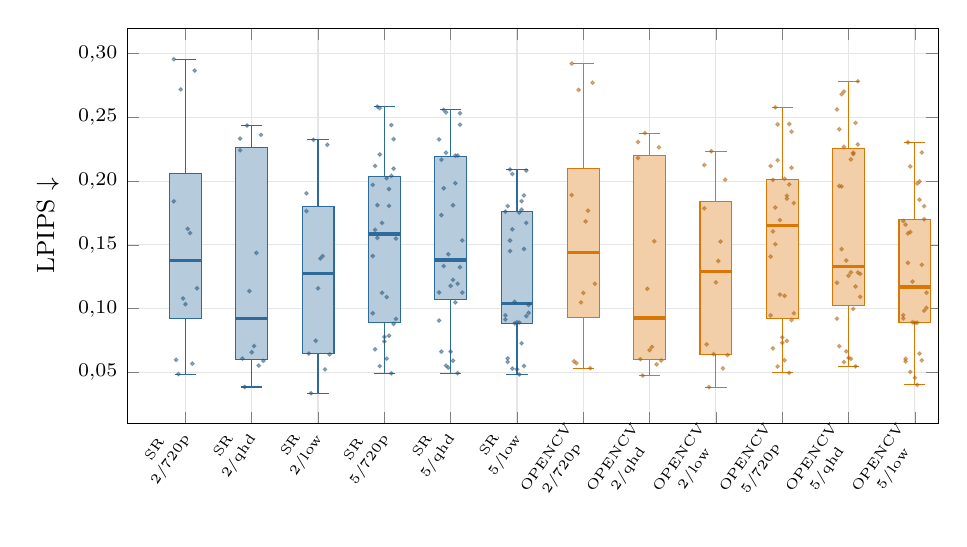
\begin{tikzpicture}
\begin{axis}[height=6.6cm,width=0.98\linewidth,enlarge x limits=0.015,xmin=-0.7,ymin=0.01,ymax=0.32,xtick=data,xticklabels={{\shortstack{SR\\2/720p}},{\shortstack{SR\\2/qhd}},{\shortstack{SR\\2/low}},{\shortstack{SR\\5/720p}},{\shortstack{SR\\5/qhd}},{\shortstack{SR\\5/low}},{\shortstack{OPENCV\\2/720p}},{\shortstack{OPENCV\\2/qhd}},{\shortstack{OPENCV\\2/low}},{\shortstack{OPENCV\\5/720p}},{\shortstack{OPENCV\\5/qhd}},{\shortstack{OPENCV\\5/low}}},x tick label style={font=\tiny,rotate=55,anchor=east},ylabel style={font=\small},tick label style={font=\scriptsize},ylabel={LPIPS $\downarrow$},grid=major,grid style={gray!20},scaled y ticks=false,ytick={0.00,0.05,0.10,0.15,0.20,0.25,0.30},yticklabels={{0,00},{0,05},{0,10},{0,15},{0,20},{0,25},{0,30}},xtick={0,1,2,3,4,5,6,7,8,9,10,11},boxplot/draw direction=y]
\draw[fill=srblue!35,draw=srblue] (axis cs:-0.2400,0.09258983) rectangle (axis cs:0.2400,0.20615650);
\draw[draw=srblue,very thick] (axis cs:-0.2400,0.13765082) -- (axis cs:0.2400,0.13765082);
\draw[draw=srblue] (axis cs:0.0000,0.04868136) -- (axis cs:0.0000,0.09258983);
\draw[draw=srblue] (axis cs:0.0000,0.20615650) -- (axis cs:0.0000,0.29572296);
\draw[draw=srblue] (axis cs:-0.1600,0.04868136) -- (axis cs:0.1600,0.04868136);
\draw[draw=srblue] (axis cs:-0.1600,0.29572296) -- (axis cs:0.1600,0.29572296);
\addplot[only marks,mark=*,mark size=0.65pt,color=srblue!80!black,opacity=0.45] coordinates {(-0.17500,0.29572296) (0.03500,0.16260658) (-0.14000,0.05985314) (0.07000,0.15928194) (-0.10500,0.04868136) (0.10500,0.05688025) (-0.07000,0.27204520) (0.14000,0.28681323) (-0.03500,0.10798584) (0.17500,0.11601970) (0.00000,0.10350206) (-0.17500,0.18419360)};
\draw[fill=srblue!35,draw=srblue] (axis cs:0.7600,0.06037673) rectangle (axis cs:1.2400,0.22656570);
\draw[draw=srblue,very thick] (axis cs:0.7600,0.09221260) -- (axis cs:1.2400,0.09221260);
\draw[draw=srblue] (axis cs:1.0000,0.03852992) -- (axis cs:1.0000,0.06037673);
\draw[draw=srblue] (axis cs:1.0000,0.22656570) -- (axis cs:1.0000,0.24364954);
\draw[draw=srblue] (axis cs:0.8400,0.03852992) -- (axis cs:1.1600,0.03852992);
\draw[draw=srblue] (axis cs:0.8400,0.24364954) -- (axis cs:1.1600,0.24364954);
\addplot[only marks,mark=*,mark size=0.65pt,color=srblue!80!black,opacity=0.45] coordinates {(0.82500,0.23341435) (1.03500,0.07064308) (0.86000,0.06081942) (1.07000,0.14372751) (0.89500,0.03852992) (1.10500,0.05533934) (0.93000,0.24364954) (1.14000,0.23631071) (0.96500,0.11378212) (1.17500,0.05904863) (1.00000,0.06579289) (0.82500,0.22428282)};
\draw[fill=srblue!35,draw=srblue] (axis cs:1.7600,0.06459939) rectangle (axis cs:2.2400,0.18005427);
\draw[draw=srblue,very thick] (axis cs:1.7600,0.12764392) -- (axis cs:2.2400,0.12764392);
\draw[draw=srblue] (axis cs:2.0000,0.03365762) -- (axis cs:2.0000,0.06459939);
\draw[draw=srblue] (axis cs:2.0000,0.18005427) -- (axis cs:2.0000,0.23248091);
\draw[draw=srblue] (axis cs:1.8400,0.03365762) -- (axis cs:2.1600,0.03365762);
\draw[draw=srblue] (axis cs:1.8400,0.23248091) -- (axis cs:2.1600,0.23248091);
\addplot[only marks,mark=*,mark size=0.65pt,color=srblue!80!black,opacity=0.45] coordinates {(1.82500,0.19051939) (2.03500,0.13936011) (1.86000,0.06475080) (2.07000,0.14123060) (1.89500,0.03365762) (2.10500,0.05233723) (1.93000,0.23248091) (2.14000,0.22851104) (1.96500,0.07480130) (2.17500,0.06414516) (2.00000,0.11592773) (1.82500,0.17656590)};
\draw[fill=srblue!35,draw=srblue] (axis cs:2.7600,0.08904129) rectangle (axis cs:3.2400,0.20372663);
\draw[draw=srblue,very thick] (axis cs:2.7600,0.15865594) -- (axis cs:3.2400,0.15865594);
\draw[draw=srblue] (axis cs:3.0000,0.04925307) -- (axis cs:3.0000,0.08904129);
\draw[draw=srblue] (axis cs:3.0000,0.20372663) -- (axis cs:3.0000,0.25853246);
\draw[draw=srblue] (axis cs:2.8400,0.04925307) -- (axis cs:3.1600,0.04925307);
\draw[draw=srblue] (axis cs:2.8400,0.25853246) -- (axis cs:3.1600,0.25853246);
\addplot[only marks,mark=*,mark size=0.65pt,color=srblue!80!black,opacity=0.45] coordinates {(2.82500,0.19708648) (3.03500,0.20237482) (2.86000,0.16180283) (3.07000,0.18061841) (2.89500,0.15550905) (3.10500,0.04925307) (2.93000,0.05490787) (3.14000,0.08806662) (2.96500,0.16728398) (3.17500,0.15497313) (3.00000,0.07784477) (2.82500,0.14128679) (3.03500,0.06075253) (2.86000,0.06808234) (3.07000,0.19389609) (2.89500,0.25853246) (3.10500,0.24400668) (2.93000,0.25729597) (3.14000,0.20982799) (2.96500,0.11243199) (3.17500,0.09196529) (3.00000,0.07429750) (2.82500,0.09637624) (3.03500,0.10907920) (2.86000,0.21198204) (3.07000,0.07876913) (2.89500,0.18125464) (3.10500,0.20417723) (2.93000,0.22092831) (3.14000,0.23304096)};
\draw[fill=srblue!35,draw=srblue] (axis cs:3.7600,0.10683540) rectangle (axis cs:4.2400,0.21922747);
\draw[draw=srblue,very thick] (axis cs:3.7600,0.13804905) -- (axis cs:4.2400,0.13804905);
\draw[draw=srblue] (axis cs:4.0000,0.04942584) -- (axis cs:4.0000,0.10683540);
\draw[draw=srblue] (axis cs:4.0000,0.21922747) -- (axis cs:4.0000,0.25596240);
\draw[draw=srblue] (axis cs:3.8400,0.04942584) -- (axis cs:4.1600,0.04942584);
\draw[draw=srblue] (axis cs:3.8400,0.25596240) -- (axis cs:4.1600,0.25596240);
\addplot[only marks,mark=*,mark size=0.65pt,color=srblue!80!black,opacity=0.45] coordinates {(3.82500,0.23272631) (4.03500,0.18109253) (3.86000,0.17334947) (4.07000,0.19845337) (3.89500,0.13337740) (4.10500,0.04942584) (3.93000,0.05527661) (4.14000,0.13253266) (3.96500,0.14272070) (4.17500,0.15355317) (4.00000,0.06629635) (3.82500,0.11273780) (4.03500,0.05913601) (3.86000,0.06629756) (4.07000,0.22001915) (3.89500,0.25596240) (4.10500,0.22011858) (3.93000,0.25402588) (4.14000,0.25332329) (3.96500,0.05368446) (4.17500,0.11260094) (4.00000,0.11788118) (3.82500,0.09068577) (4.03500,0.12255567) (3.86000,0.21685244) (4.07000,0.10491355) (3.89500,0.19445321) (4.10500,0.11951250) (3.93000,0.22231930) (4.14000,0.24430104)};
\draw[fill=srblue!35,draw=srblue] (axis cs:4.7600,0.08864863) rectangle (axis cs:5.2400,0.17592043);
\draw[draw=srblue,very thick] (axis cs:4.7600,0.10415204) -- (axis cs:5.2400,0.10415204);
\draw[draw=srblue] (axis cs:5.0000,0.04839443) -- (axis cs:5.0000,0.08864863);
\draw[draw=srblue] (axis cs:5.0000,0.17592043) -- (axis cs:5.0000,0.20916155);
\draw[draw=srblue] (axis cs:4.8400,0.04839443) -- (axis cs:5.1600,0.04839443);
\draw[draw=srblue] (axis cs:4.8400,0.20916155) -- (axis cs:5.1600,0.20916155);
\addplot[only marks,mark=*,mark size=0.65pt,color=srblue!80!black,opacity=0.45] coordinates {(4.82500,0.17610496) (5.03500,0.17536683) (4.86000,0.18045580) (5.07000,0.17764093) (4.89500,0.15347970) (5.10500,0.05502026) (4.93000,0.05294246) (5.14000,0.09411658) (4.96500,0.10541567) (5.17500,0.10288841) (5.00000,0.05245670) (4.82500,0.09479292) (5.03500,0.04839443) (4.86000,0.05818321) (5.07000,0.18431392) (4.89500,0.20916155) (5.10500,0.18886134) (4.93000,0.20565924) (5.14000,0.20838067) (4.96500,0.08850907) (5.17500,0.09668281) (5.00000,0.08935268) (4.82500,0.09151858) (5.03500,0.08906731) (4.86000,0.06096105) (5.07000,0.07287082) (4.89500,0.14517997) (5.10500,0.14681292) (4.93000,0.16227931) (5.14000,0.16730070)};
\draw[fill=opencvorange!35,draw=opencvorange] (axis cs:5.7600,0.09335632) rectangle (axis cs:6.2400,0.20973054);
\draw[draw=opencvorange,very thick] (axis cs:5.7600,0.14397968) -- (axis cs:6.2400,0.14397968);
\draw[draw=opencvorange] (axis cs:6.0000,0.05330852) -- (axis cs:6.0000,0.09335632);
\draw[draw=opencvorange] (axis cs:6.0000,0.20973054) -- (axis cs:6.0000,0.29230875);
\draw[draw=opencvorange] (axis cs:5.8400,0.05330852) -- (axis cs:6.1600,0.05330852);
\draw[draw=opencvorange] (axis cs:5.8400,0.29230875) -- (axis cs:6.1600,0.29230875);
\addplot[only marks,mark=*,mark size=0.65pt,color=opencvorange!80!black,opacity=0.45] coordinates {(5.82500,0.29230875) (6.03500,0.16843995) (5.86000,0.05870277) (6.07000,0.17682393) (5.89500,0.05724720) (6.10500,0.05330852) (5.93000,0.27165464) (6.14000,0.27724850) (5.96500,0.10490750) (6.17500,0.11951941) (6.00000,0.11235405) (5.82500,0.18908918)};
\draw[fill=opencvorange!35,draw=opencvorange] (axis cs:6.7600,0.06009920) rectangle (axis cs:7.2400,0.22030045);
\draw[draw=opencvorange,very thick] (axis cs:6.7600,0.09274324) -- (axis cs:7.2400,0.09274324);
\draw[draw=opencvorange] (axis cs:7.0000,0.04750333) -- (axis cs:7.0000,0.06009920);
\draw[draw=opencvorange] (axis cs:7.0000,0.22030045) -- (axis cs:7.0000,0.23774353);
\draw[draw=opencvorange] (axis cs:6.8400,0.04750333) -- (axis cs:7.1600,0.04750333);
\draw[draw=opencvorange] (axis cs:6.8400,0.23774353) -- (axis cs:7.1600,0.23774353);
\addplot[only marks,mark=*,mark size=0.65pt,color=opencvorange!80!black,opacity=0.45] coordinates {(6.82500,0.23070115) (7.03500,0.06994356) (6.86000,0.06034965) (7.07000,0.15293080) (6.89500,0.04750333) (7.10500,0.05625489) (6.93000,0.23774353) (7.14000,0.22659498) (6.96500,0.11554292) (7.17500,0.05934786) (7.00000,0.06750482) (6.82500,0.21820228)};
\draw[fill=opencvorange!35,draw=opencvorange] (axis cs:7.7600,0.06410739) rectangle (axis cs:8.2400,0.18436639);
\draw[draw=opencvorange,very thick] (axis cs:7.7600,0.12898952) -- (axis cs:8.2400,0.12898952);
\draw[draw=opencvorange] (axis cs:8.0000,0.03848322) -- (axis cs:8.0000,0.06410739);
\draw[draw=opencvorange] (axis cs:8.0000,0.18436639) -- (axis cs:8.0000,0.22348472);
\draw[draw=opencvorange] (axis cs:7.8400,0.03848322) -- (axis cs:8.1600,0.03848322);
\draw[draw=opencvorange] (axis cs:7.8400,0.22348472) -- (axis cs:8.1600,0.22348472);
\addplot[only marks,mark=*,mark size=0.65pt,color=opencvorange!80!black,opacity=0.45] coordinates {(7.82500,0.17875841) (8.03500,0.13735849) (7.86000,0.07201471) (8.07000,0.15264787) (7.89500,0.03848322) (8.10500,0.05321711) (7.93000,0.22348472) (8.14000,0.20119034) (7.96500,0.06429386) (8.17500,0.06354798) (8.00000,0.12062056) (7.82500,0.21265669)};
\draw[fill=opencvorange!35,draw=opencvorange] (axis cs:8.7600,0.09197107) rectangle (axis cs:9.2400,0.20162609);
\draw[draw=opencvorange,very thick] (axis cs:8.7600,0.16506689) -- (axis cs:9.2400,0.16506689);
\draw[draw=opencvorange] (axis cs:9.0000,0.04958973) -- (axis cs:9.0000,0.09197107);
\draw[draw=opencvorange] (axis cs:9.0000,0.20162609) -- (axis cs:9.0000,0.25789511);
\draw[draw=opencvorange] (axis cs:8.8400,0.04958973) -- (axis cs:9.1600,0.04958973);
\draw[draw=opencvorange] (axis cs:8.8400,0.25789511) -- (axis cs:9.1600,0.25789511);
\addplot[only marks,mark=*,mark size=0.65pt,color=opencvorange!80!black,opacity=0.45] coordinates {(8.82500,0.21188551) (9.03500,0.20184442) (8.86000,0.16060756) (9.07000,0.18858510) (8.89500,0.15056062) (9.10500,0.04958973) (8.93000,0.05459280) (9.14000,0.09104508) (8.96500,0.16952622) (9.17500,0.18284756) (9.00000,0.07749642) (8.82500,0.14085862) (9.03500,0.05956749) (8.86000,0.06888153) (9.07000,0.18624356) (8.89500,0.25789511) (9.10500,0.24485075) (8.93000,0.24458295) (9.14000,0.21054018) (8.96500,0.11101067) (9.17500,0.09639119) (9.00000,0.07324846) (8.82500,0.09474902) (9.03500,0.11002779) (8.86000,0.20097110) (9.07000,0.07473231) (8.89500,0.17938712) (9.10500,0.19744457) (8.93000,0.21643001) (9.14000,0.23884936)};
\draw[fill=opencvorange!35,draw=opencvorange] (axis cs:9.7600,0.10217504) rectangle (axis cs:10.2400,0.22576700);
\draw[draw=opencvorange,very thick] (axis cs:9.7600,0.13315308) -- (axis cs:10.2400,0.13315308);
\draw[draw=opencvorange] (axis cs:10.0000,0.05477412) -- (axis cs:10.0000,0.10217504);
\draw[draw=opencvorange] (axis cs:10.0000,0.22576700) -- (axis cs:10.0000,0.27841073);
\draw[draw=opencvorange] (axis cs:9.8400,0.05477412) -- (axis cs:10.1600,0.05477412);
\draw[draw=opencvorange] (axis cs:9.8400,0.27841073) -- (axis cs:10.1600,0.27841073);
\addplot[only marks,mark=*,mark size=0.65pt,color=opencvorange!80!black,opacity=0.45] coordinates {(9.82500,0.25630644) (10.03500,0.21711023) (9.86000,0.19620068) (10.07000,0.22228009) (9.89500,0.14671056) (10.10500,0.05477412) (9.93000,0.05812582) (10.14000,0.12836577) (9.96500,0.13781993) (10.17500,0.12722649) (10.00000,0.06144616) (9.82500,0.12030654) (10.03500,0.06064026) (9.86000,0.07057868) (10.07000,0.22132519) (9.89500,0.26819271) (10.10500,0.24577163) (9.93000,0.27025598) (10.14000,0.27841073) (9.96500,0.06650098) (10.17500,0.10929263) (10.00000,0.12580912) (9.82500,0.09216833) (10.03500,0.12848623) (9.86000,0.24076509) (10.07000,0.09980251) (9.89500,0.19584025) (10.10500,0.11736227) (9.93000,0.22692931) (10.14000,0.22882980)};
\draw[fill=opencvorange!35,draw=opencvorange] (axis cs:10.7600,0.08889340) rectangle (axis cs:11.2400,0.16984769);
\draw[draw=opencvorange,very thick] (axis cs:10.7600,0.11689767) -- (axis cs:11.2400,0.11689767);
\draw[draw=opencvorange] (axis cs:11.0000,0.04018669) -- (axis cs:11.0000,0.08889340);
\draw[draw=opencvorange] (axis cs:11.0000,0.16984769) -- (axis cs:11.0000,0.23045835);
\draw[draw=opencvorange] (axis cs:10.8400,0.04018669) -- (axis cs:11.1600,0.04018669);
\draw[draw=opencvorange] (axis cs:10.8400,0.23045835) -- (axis cs:11.1600,0.23045835);
\addplot[only marks,mark=*,mark size=0.65pt,color=opencvorange!80!black,opacity=0.45] coordinates {(10.82500,0.16880244) (11.03500,0.19816342) (10.86000,0.16587561) (11.07000,0.19978732) (10.89500,0.15901878) (11.10500,0.05948650) (10.93000,0.05040193) (11.14000,0.09837994) (10.96500,0.12127320) (11.17500,0.11252214) (11.00000,0.04577556) (10.82500,0.09491450) (11.03500,0.04018669) (10.86000,0.05856302) (11.07000,0.18542700) (10.89500,0.23045835) (11.10500,0.22249496) (10.93000,0.21157633) (11.14000,0.18035024) (10.96500,0.08932389) (11.17500,0.10063782) (11.00000,0.08887595) (10.82500,0.09233965) (11.03500,0.08894576) (10.86000,0.06063940) (11.07000,0.06473484) (10.89500,0.13593188) (11.10500,0.13442613) (10.93000,0.16009068) (11.14000,0.17019610)};
\end{axis}
\end{tikzpicture}
\par\vspace{3pt}
\vspace{3pt}
\begin{minipage}{0.98\linewidth}\scriptsize Jeder Punkt ist eine einzelne Evaluationsansicht aus \texttt{per\_frame} und liegt bewusst auf der zentralen x-Kategorie der zugehörigen Box; die Box zeigt Quartile und robuste 1,5-IQR-Whisker. Die STS-Boxplots enthalten nur vollständige Original-GS-A-Routen; die SuGaR-Boxplots enthalten alle zwölf vollständigen Coarse-Läufe. Die x-Beschriftung kodiert Kamera, FPS und Auflösung; es gibt deshalb keine separate Kamera-Legende. Unterschiedliche Auflösungen bleiben als separate Konfigurationen gekennzeichnet und werden nicht zu einer globalen Rangliste zusammengefasst.\end{minipage}
\end{center}
\end{document}